\chapter{STrans 智慧交通视觉感知与管理系统需求分析报告 V2.0}\label{requirements-strans-ux667aux6167ux4ea4ux901aux89c6ux89c9ux611fux77e5ux4e0eux7ba1ux7406ux7cfbux7edfux9700ux6c42ux5206ux6790ux62a5ux544a-v2.0}

\section{文档信息}\label{requirements-ux6587ux6863ux4fe1ux606f}

\begin{longtable}[]{@{}ll@{}}
\toprule\noalign{}
项目 & 内容 \\
\midrule\noalign{}
\endhead
\bottomrule\noalign{}
\endlastfoot
项目名称 & 基于多源视觉感知的智慧交通沙盘监测与分析系统 \\
软件名称 & STrans（Smart Transportation Sensing System） \\
文档版本 & V2.0 \\
编制日期 & 2026-07-14 \\
需求基线 & 《软件工程实训II-包老师.pdf》、\texttt{需求分析文档\_\allowbreak{}\allowbreak{}V1.\allowbreak{}0.\allowbreak{}md} \\
实现基线 & \texttt{L\allowbreak{}I\allowbreak{}N\allowbreak{}G} 分支 \texttt{b0f3be2} 及当前结题工作区 \\
文档状态 & 结题交付版 \\
\end{longtable}

本文用于定义 STrans 的最终交付需求、验收口径和成果边界。V2.0 以课程初始要求为目标基线，以当前代码、自动化测试、浏览器遍历和真实沙盘视频为事实依据。文中``已实现''\,``部分满足''和``后续项''必须严格区分，测试通过率不等同于需求覆盖率或算法准确率。

\section{版本变更记录}\label{requirements-ux7248ux672cux53d8ux66f4ux8bb0ux5f55}

\begin{longtable}[]{@{}
  >{\raggedright\arraybackslash}p{(\linewidth - 4\tabcolsep) * \real{0.3333}}
  >{\raggedright\arraybackslash}p{(\linewidth - 4\tabcolsep) * \real{0.3333}}
  >{\raggedright\arraybackslash}p{(\linewidth - 4\tabcolsep) * \real{0.3333}}@{}}
\toprule\noalign{}
\begin{minipage}[b]{\linewidth}\raggedright
版本
\end{minipage} & \begin{minipage}[b]{\linewidth}\raggedright
日期
\end{minipage} & \begin{minipage}[b]{\linewidth}\raggedright
主要内容
\end{minipage} \\
\midrule\noalign{}
\endhead
\bottomrule\noalign{}
\endlastfoot
V1.0 & 2026-07-06 & 建立云边端协同、车辆检测、车牌、拥堵、异常和 Web 展示的初始需求基线 \\
V2.0 & 2026-07-14 & 按当前实现重构需求边界；前端统一为 React；通信主链路统一为 MJPEG + REST；补充认证授权、证据链、自适应调度、道路建模和真实数据验收；移除已退出采集方案；将未实现的碰撞识别、信号灯识别和完整跨线统计移出交付范围 \\
\end{longtable}

V2.0 的核心变化不是增加设想，而是把初始要求转换为可追踪、可验收且与现有软件一致的最终需求。

\section{项目背景与问题定义}\label{requirements-ux9879ux76eeux80ccux666fux4e0eux95eeux9898ux5b9aux4e49}

课程要求面向智慧交通沙盘构建视频采集、计算分析和前端展示相协同的视觉感知系统，并重点完成车牌与白名单决策、车辆密度与拥堵热力、禁停车辆告警、道路异常告警以及设备、模型、资源和历史管理。

沙盘场景具有车辆目标小、遮挡多、车牌像素少、路面反光和标线显著等特点；同时，RTSP、MJPEG、手机/USB 摄像头、本地图片和录像的输入形式不统一。单独运行识别脚本无法满足用户权限、历史查询、告警处置和证据留存等软件工程要求。因此，本项目需要解决以下问题：

\begin{enumerate}
\def\labelenumi{\arabic{enumi}.}
\tightlist
\item
  将多源视频统一接入稳定、可切换的分析链路；
\item
  将单帧识别结果稳定为车辆轨迹、车牌和交通状态；
\item
  将像素坐标转换为车道、路口、禁停和拥堵等道路语义；
\item
  在有限标注数据下提供可解释的道路异常候选检测；
\item
  将识别、告警、处置、历史、证据和审计形成闭环。
\end{enumerate}

\section{建设目标}\label{requirements-ux5efaux8bbeux76eeux6807}

\begin{itemize}
\tightlist
\item
  建立网络视频、手机/USB 摄像头、本地图片和录像的统一接入与管理能力；
\item
  完成车辆检测与跟踪、车牌识别和白名单软件决策；
\item
  完成车辆数量、密度、参考速度、禁停和拥堵热力分析；
\item
  完成道路异物、道路行人和可选道路破损候选检测；
\item
  建立二维道路建模、摄像头标定和道路空间映射能力；
\item
  提供 Web 实时监控、系统资源、模型参数、历史、告警、证据和审计功能；
\item
  使用自动化测试、浏览器检查和真实沙盘视频形成可复核的结题证据。
\end{itemize}

\section{利益相关者}\label{requirements-ux5229ux76caux76f8ux5173ux8005}

\begin{longtable}[]{@{}
  >{\raggedright\arraybackslash}p{(\linewidth - 4\tabcolsep) * \real{0.3333}}
  >{\raggedright\arraybackslash}p{(\linewidth - 4\tabcolsep) * \real{0.3333}}
  >{\raggedright\arraybackslash}p{(\linewidth - 4\tabcolsep) * \real{0.3333}}@{}}
\toprule\noalign{}
\begin{minipage}[b]{\linewidth}\raggedright
利益相关者
\end{minipage} & \begin{minipage}[b]{\linewidth}\raggedright
关注点
\end{minipage} & \begin{minipage}[b]{\linewidth}\raggedright
对系统的期望
\end{minipage} \\
\midrule\noalign{}
\endhead
\bottomrule\noalign{}
\endlastfoot
课程教师/验收人员 & 需求准确性、方案合理性、功能效果、创新性和成果物质量 & 在规定时间内看到可重复演示、真实效果、测试证据和诚实边界 \\
普通用户/监控人员 & 实时态势、告警、历史和操作便利性 & 登录后快速查看视频、识别结果、热力图、事件和报告 \\
系统管理员 & 配置、权限、设备、模型、数据和审计 & 可管理摄像头、用户、白名单、参数、调度和道路模型 \\
算法工程人员 & 输入质量、模型配置、性能和失败样本 & 可复现实验环境，获得结构化结果和真实误报/漏报样本 \\
部署维护人员 & 环境依赖、故障恢复、数据安全和备份 & 有明确启动、监控、降级、备份与故障处理说明 \\
视频源/外部服务 & 接口兼容、超时和降级 & 通过受控接口提供视频、远程算法或智能报告能力 \\
\end{longtable}

\section{系统范围}\label{requirements-ux7cfbux7edfux8303ux56f4}

\subsection{纳入交付范围}\label{requirements-ux7eb3ux5165ux4ea4ux4ed8ux8303ux56f4}

\begin{itemize}
\tightlist
\item
  多源视频配置、连通性测试、启停、状态和 MJPEG 展示；
\item
  车辆检测、ByteTrack 跟踪、去重、平滑和短时稳定；
\item
  HyperLPR3 车牌识别、多帧稳定、白名单查询和 \texttt{allow/\allowbreak{}deny} 软件决策；
\item
  当前车辆数、密度、参考视角速度估计、禁停和拥堵热力；
\item
  道路异物、道路行人及可选道路破损候选；
\item
  SegFormer 道路掩膜、摄像头单应标定、车道/路口归属；
\item
  二维道路拓扑、摄像头和标定关系的可视化建模及 JSON 导出；
\item
  React Web 大屏、认证授权、摄像头/模型/白名单/用户管理；
\item
  SQLite 历史、告警处置、证据包、SHA-256 完整性清单和审计；
\item
  CPU、内存、GPU、显存和推理耗时监控及自适应调度；
\item
  可选远程算法、天气和智能报告服务，外部服务失败不阻断核心链路。
\end{itemize}

\subsection{不纳入当前交付范围}\label{requirements-ux4e0dux7eb3ux5165ux5f53ux524dux4ea4ux4ed8ux8303ux56f4}

\begin{itemize}
\tightlist
\item
  物理闸机或其他道路硬件的实际控制；
\item
  独立交通碰撞/事故识别模型；
\item
  信号灯状态识别主链路；
\item
  完整的跨线进入/离开流量算法；
\item
  多摄像头身份融合和跨镜跟踪；
\item
  完整三维数字孪生、自动路径规划和信号灯控制；
\item
  无人工真值条件下的严格 Precision、Recall、F1 或整牌准确率承诺；
\item
  面向生产环境的多节点高可用、长周期压力和公网安全认证。
\end{itemize}

\pandocbounded{\includegraphics[keepaspectratio,alt={系统组件与边界关系}]{assets/component-architecture.png}}

\textbf{图 6-1 系统组件与需求边界。} 图中以视频接入、视觉感知、道路逻辑、业务存储、API 和 React 展示构成当前交付主链路，道路建模工具通过配置产物支撑空间分析。该图用于说明功能需求落在哪些系统边界内，并不单独证明组件运行正确；运行性仍须由自动化测试、浏览器检查和真实视频记录共同证明，可选外部服务也不属于核心链路的强依赖。

\section{角色与权限}\label{requirements-ux89d2ux8272ux4e0eux6743ux9650}

\begin{longtable}[]{@{}
  >{\raggedright\arraybackslash}p{(\linewidth - 2\tabcolsep) * \real{0.5000}}
  >{\raggedright\arraybackslash}p{(\linewidth - 2\tabcolsep) * \real{0.5000}}@{}}
\toprule\noalign{}
\begin{minipage}[b]{\linewidth}\raggedright
角色
\end{minipage} & \begin{minipage}[b]{\linewidth}\raggedright
核心权限
\end{minipage} \\
\midrule\noalign{}
\endhead
\bottomrule\noalign{}
\endlastfoot
未登录访问者 & 获取验证码、注册、登录；不能访问业务和管理数据 \\
普通用户 & 查看和启动摄像头、实时识别、热力图、历史、告警、报告和白名单；修改本人密码；按现有接口处置告警与下载证据 \\
管理员 & 具备普通用户权限，并可管理摄像头、用户、白名单、模型配置、自适应调度、智能报告配置、审计和道路建模入口 \\
外部视频源 & 提供视频帧，不拥有业务操作权限 \\
可选算法/报告服务 & 仅通过约定接口返回结果，不直接访问用户管理和业务数据库 \\
\end{longtable}

完整系统参与者和用例关系见 \href{diagrams/use-case.puml}{用例图}，答辩精简版见 \href{diagrams/use-case-overview.puml}{用例概览图}。

\pandocbounded{\includegraphics[keepaspectratio,alt={系统核心用例概览}]{assets/use-case-overview.png}}

\textbf{图 7-1 系统核心用例概览。} 普通用户围绕实时监控、识别结果和数据查询开展业务操作，管理员在此基础上承担视频源、模型、账号、白名单和道路配置职责。该图是需求层的参与者---用例摘要，不表示每一个用例均已获得同等深度的自动化覆盖；各用例的实际完成度应以第 8 节状态和第 13 节追踪矩阵为准。

\section{功能需求}\label{requirements-ux529fux80fdux9700ux6c42}

\subsection{功能需求总表}\label{requirements-ux529fux80fdux9700ux6c42ux603bux8868}

优先级采用 P0（结题必须）、P1（重要支撑）和 P2（增强）。状态采用``功能级满足、部分满足、后续项''。

\begin{longtable}[]{@{}
  >{\raggedright\arraybackslash}p{(\linewidth - 6\tabcolsep) * \real{0.2143}}
  >{\raggedright\arraybackslash}p{(\linewidth - 6\tabcolsep) * \real{0.2143}}
  >{\centering\arraybackslash}p{(\linewidth - 6\tabcolsep) * \real{0.3571}}
  >{\raggedright\arraybackslash}p{(\linewidth - 6\tabcolsep) * \real{0.2143}}@{}}
\toprule\noalign{}
\begin{minipage}[b]{\linewidth}\raggedright
ID
\end{minipage} & \begin{minipage}[b]{\linewidth}\raggedright
功能需求
\end{minipage} & \begin{minipage}[b]{\linewidth}\centering
优先级
\end{minipage} & \begin{minipage}[b]{\linewidth}\raggedright
当前状态
\end{minipage} \\
\midrule\noalign{}
\endhead
\bottomrule\noalign{}
\endlastfoot
R-01 & 多源视频采集、计算分析与浏览器展示形成协同链路 & P0 & 部分满足 \\
R-02 & 支持智慧交通沙盘真实视频场景 & P0 & 功能级满足 \\
R-03 & 车牌识别、白名单比较和通行软件决策 & P0 & 部分满足 \\
R-04 & 车辆检测、区域数量/密度和拥堵热力图 & P0 & 部分满足 \\
R-05 & 禁停区域车辆跟踪、停留判定和告警 & P0 & 部分满足 \\
R-06 & 道路异常物候选、位置和道路语义关联 & P0 & 部分满足 \\
R-07 & CPU、GPU、内存、视频和推理状态监控 & P1 & 功能级满足 \\
R-08 & 视频源设备注册、配置、启停和状态管理 & P0 & 部分满足 \\
R-09 & 模型选择、阈值配置和资源自适应调度 & P1 & 功能级满足 \\
R-10 & 闸机决策、热力、禁停和道路监控统一展示 & P0 & 部分满足 \\
R-11 & 历史统计、告警处置、证据、导出和审计 & P0 & 部分满足 \\
R-12 & 二维道路空间与摄像头标定可视化配置 & P1 & 功能级满足（扩展） \\
\end{longtable}

\subsection{详细功能要求与验收标准}\label{requirements-ux8be6ux7ec6ux529fux80fdux8981ux6c42ux4e0eux9a8cux6536ux6807ux51c6}

\subsubsection{R-01 多源协同链路}\label{requirements-r-01-ux591aux6e90ux534fux540cux94feux8def}

\begin{itemize}
\tightlist
\item
  系统应统一接入 RTSP/MJPEG、手机/USB 摄像头、本地图片和录像；
\item
  后端应向浏览器提供原始和模型标注 MJPEG，并通过 REST 提供结构化结果；
\item
  视频源或可选外部服务不可用时，核心 Web 系统不得整体崩溃；
\item
  验收以部署图、真实视频启动、模型流显示和状态查询为证据；当前不宣称已完成三台独立物理节点的长稳验收。
\end{itemize}

\subsubsection{R-02 真实沙盘场景}\label{requirements-r-02-ux771fux5b9eux6c99ux76d8ux573aux666f}

\begin{itemize}
\tightlist
\item
  系统应能读取真实沙盘录像，并保留来源、采样和运行环境信息；
\item
  演示素材应来自真实录像或实时流，不以合成结果冒充真实识别；
\item
  验收以 13 段视频、65 帧 CUDA 批量结果和前端实时流记录为证据。
\end{itemize}

\pandocbounded{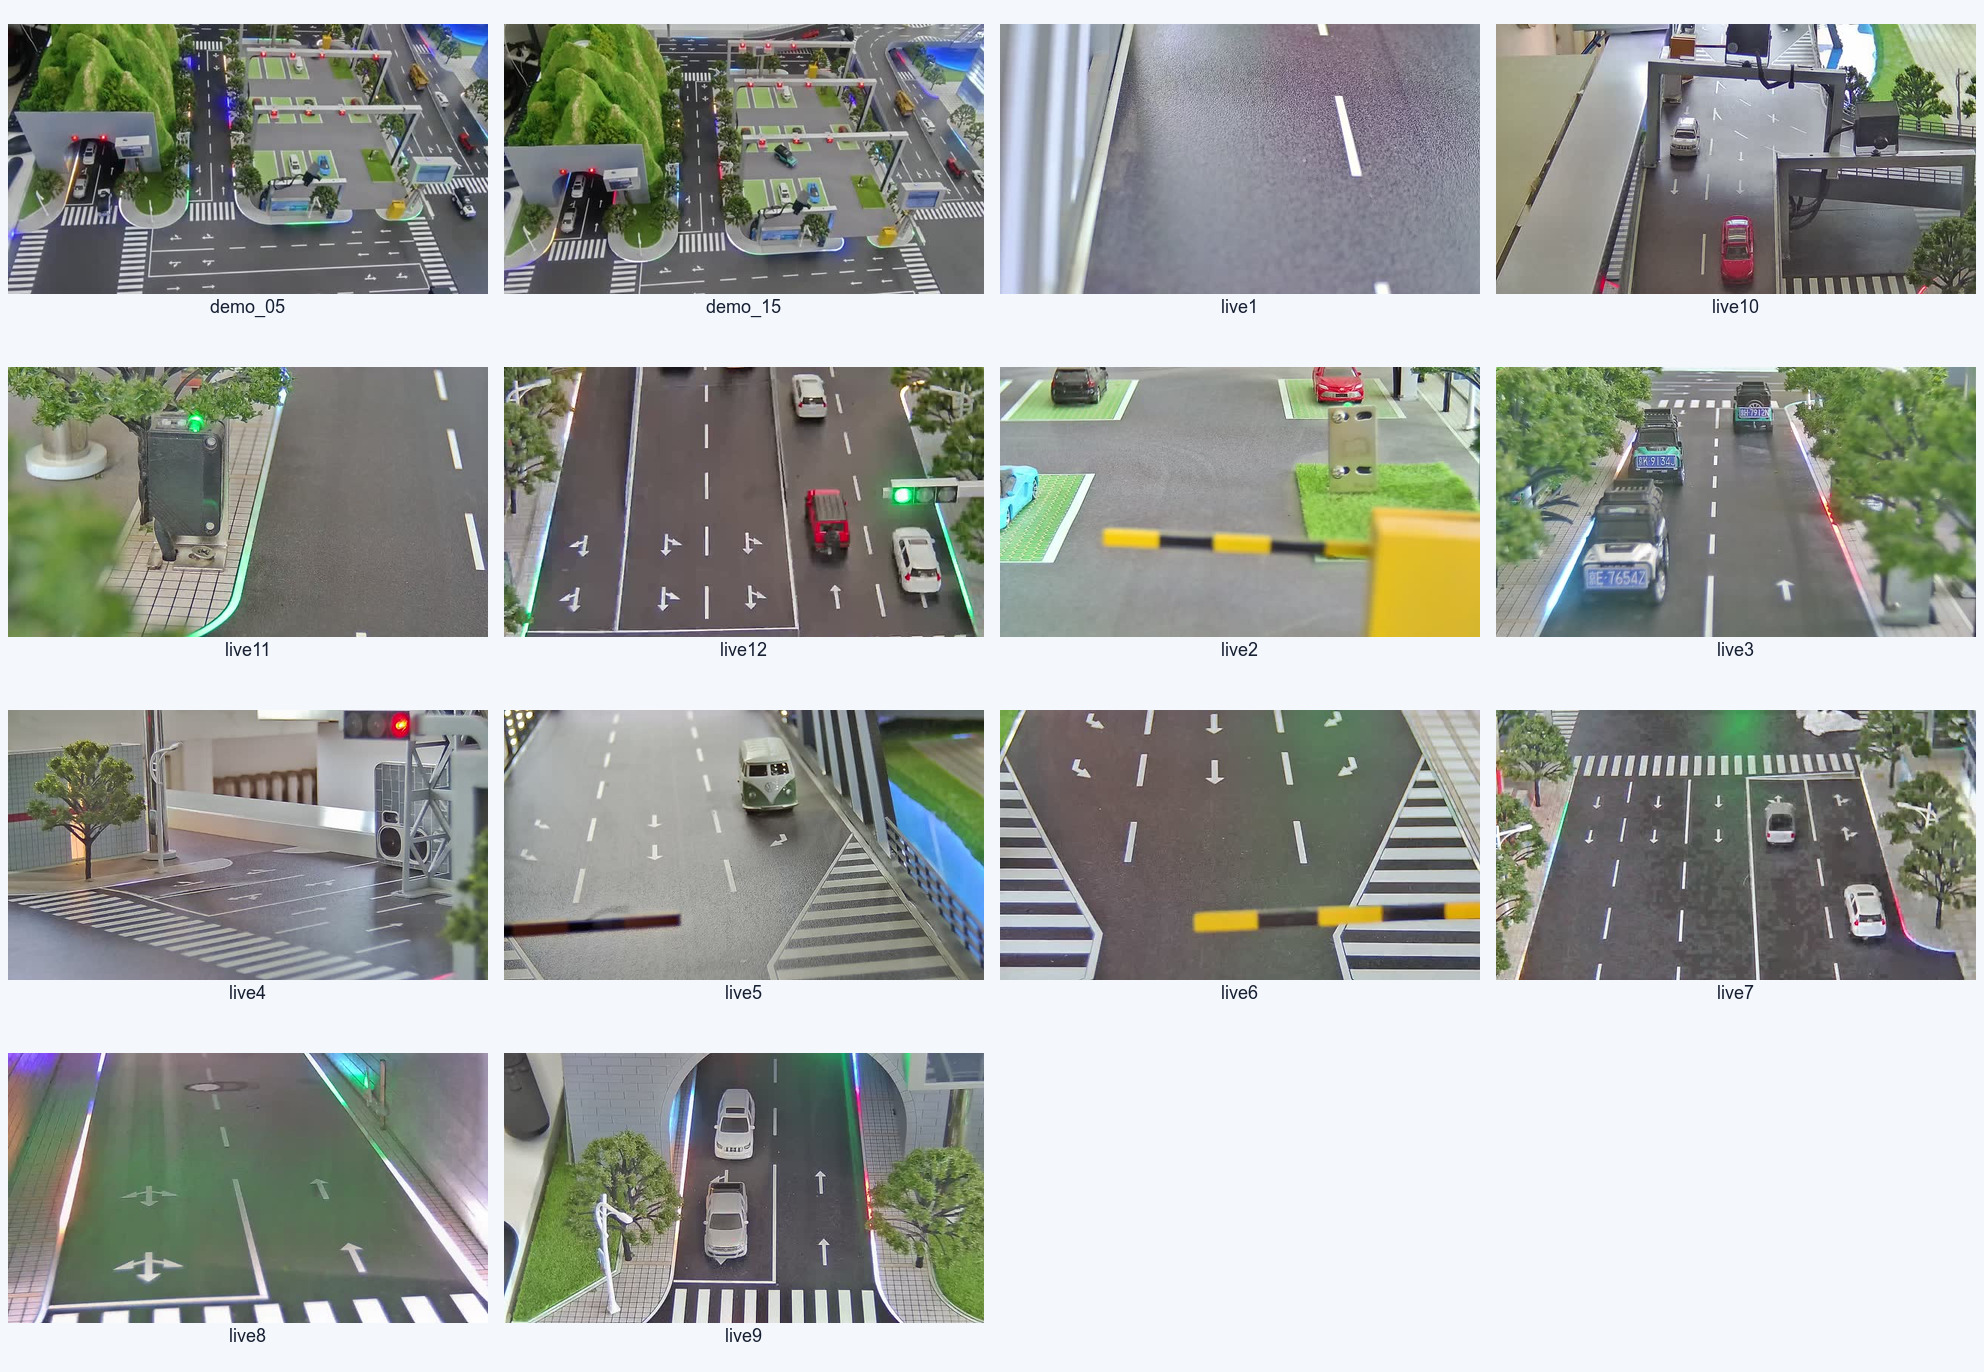
\includegraphics[keepaspectratio,alt={真实沙盘视频数据集总览}]{assets/dataset-inventory-contact-sheet.jpg}}

\textbf{图 8-1 真实沙盘视频数据集总览。} 联系表用于证明评测输入覆盖多路沙盘机位和不同道路画面，也是后续建立分层真值集的素材基线。图中画面只能证明数据来源与场景覆盖，不能直接证明车辆、车牌或异常识别准确率；在未完成逐帧人工标注前，第 12、13 节仅引用系统输出数量和运行耗时。

\subsubsection{R-03 车牌与白名单决策}\label{requirements-r-03-ux8f66ux724cux4e0eux767dux540dux5355ux51b3ux7b56}

\begin{itemize}
\tightlist
\item
  系统应对车辆区域执行 OCR，并允许周期性全帧识别补充漏检；
\item
  车牌文本应与车辆轨迹关联，经规范化和多帧稳定后再查询白名单；
\item
  输出应包含车牌、置信信息、白名单状态、\texttt{allow/\allowbreak{}deny} 和原因；
\item
  决策仅为软件建议，不驱动物理设备；未完成真值标注前不得声称整牌准确率达标。
\end{itemize}

\subsubsection{R-04 车辆、密度与拥堵}\label{requirements-r-04-ux8f66ux8f86ux5bc6ux5ea6ux4e0eux62e5ux5835}

\begin{itemize}
\tightlist
\item
  系统应输出车辆检测框、类别、置信度和可用的跟踪 ID；
\item
  应通过 ROI、几何、去重和平滑减少沙盘误检和抖动；
\item
  应根据近期活跃唯一轨迹输出当前数量、密度和道路/路口拥堵状态；
\item
  热力图应支持关闭、画面叠加和道路示意模式；
\item
  \texttt{count\_\allowbreak{}in/\allowbreak{}count\_\allowbreak{}out} 仅为接口兼容字段，不作为完整跨线统计成果。
\end{itemize}

\subsubsection{R-05 禁停告警}\label{requirements-r-05-ux7981ux505cux544aux8b66}

\begin{itemize}
\tightlist
\item
  已标定摄像头应将车辆接地点映射到道路坐标，并判断是否处于禁停区域；
\item
  同一轨迹持续停留超过阈值时应产生 \texttt{no\_\allowbreak{}stop} 事件；
\item
  验收至少覆盖点位/区域、停留状态和事件结构的确定性测试；
\item
  当前缺少专项真实禁停长视频，状态为部分满足。
\end{itemize}

\subsubsection{R-06 道路异常}\label{requirements-r-06-ux9053ux8defux5f02ux5e38}

\begin{itemize}
\tightlist
\item
  道路异常任务应与车辆监控任务隔离，不得把异常框计入车辆统计；
\item
  应结合道路 ROI、背景变化、相机运动、合法车辆/行人解释、外观和多帧一致性输出候选；
\item
  结果至少区分道路异物、道路行人和可选道路破损候选，并保留位置；
\item
  当前结果定位为``候选检测 + 人工复核''；道路标线误报和同类事件重复必须作为已知问题披露。
\end{itemize}

\subsubsection{R-07 资源与运行监控}\label{requirements-r-07-ux8d44ux6e90ux4e0eux8fd0ux884cux76d1ux63a7}

\begin{itemize}
\tightlist
\item
  系统应显示 CPU、内存、GPU、显存、推理耗时和视频状态；
\item
  GPU 不可用时应明确显示并允许 CPU 降级；
\item
  指标用于运行诊断和调度，不得把视频解码帧率与综合分析更新率混为一谈。
\end{itemize}

\subsubsection{R-08 视频源设备管理}\label{requirements-r-08-ux89c6ux9891ux6e90ux8bbeux5907ux7ba1ux7406}

\begin{itemize}
\tightlist
\item
  管理员应能新增、修改、删除、测试、启动和停止视频源；
\item
  系统应显示在线/离线、来源类型、位置和连接状态；
\item
  日志、状态和审计不得暴露完整带凭据地址；
\item
  当前实现以``摄像头/视频源''作为设备抽象，未建立独立边缘计算节点心跳协议。
\end{itemize}

\subsubsection{R-09 模型配置与调度}\label{requirements-r-09-ux6a21ux578bux914dux7f6eux4e0eux8c03ux5ea6}

\begin{itemize}
\tightlist
\item
  管理员应能配置模型标识、置信度、输入尺寸、检测间隔和任务模式；
\item
  自适应调度应根据任务、来源类型、CPU、内存、GPU、显存和耗时选择策略；
\item
  应支持 quality、balanced、realtime、protect、anomaly 和 manual 档位，并避免非必要频繁切换；
\item
  不同模型精度/速度对比需在统一真值集建立后另行验收。
\end{itemize}

\subsubsection{R-10 统一监控展示}\label{requirements-r-10-ux7edfux4e00ux76d1ux63a7ux5c55ux793a}

\begin{itemize}
\tightlist
\item
  实时页面应展示原始/标注画面、车辆与车牌、白名单决策、交通状态、热力和事件；
\item
  普通用户与管理员应看到与角色匹配的操作入口；
\item
  后端不可用时页面应保留可理解的离线或错误状态；
\item
  四类场景已有软件入口，但仍需在正式演示脚本中逐项核验。
\end{itemize}

\pandocbounded{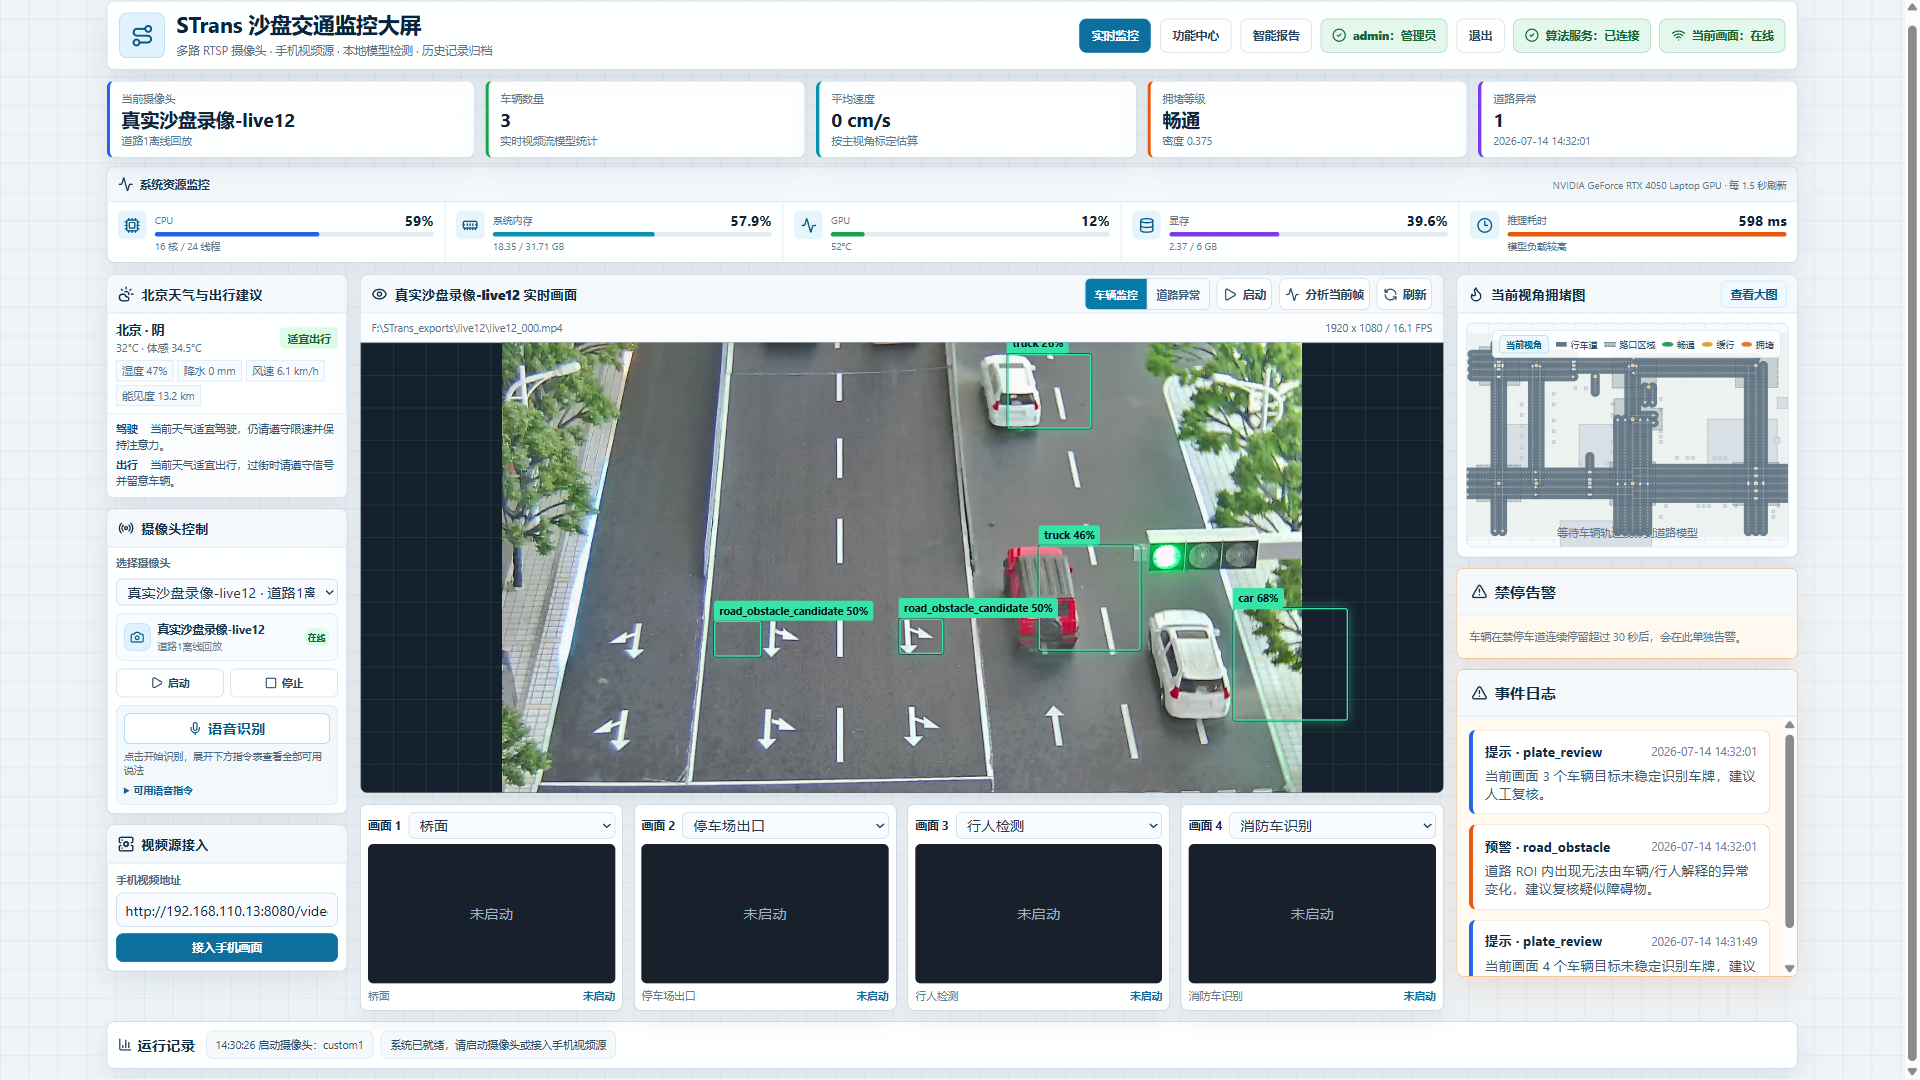
\includegraphics[keepaspectratio,alt={真实视频在前端实时监控页面中的运行画面}]{assets/frontend-realtime-live12.png}}

\textbf{图 8-2 前端真实流运行证据。} 该截图展示真实沙盘录像经视频接入、模型分析和 Web 展示后的集成状态，可作为 R-01、R-04 和 R-10 的浏览器侧证据。截图反映的是特定设备、模型、阈值和时刻的运行结果，不代表所有机位均达到相同效果，也不能替代连续运行、人工真值或权限矩阵测试。

\subsubsection{R-11 数据闭环}\label{requirements-r-11-ux6570ux636eux95edux73af}

\begin{itemize}
\tightlist
\item
  结构化分析结果和事件应写入 SQLite，并支持历史查询、筛选和 CSV/JSON 导出；
\item
  告警应支持状态、处理人和备注；证据包应包含原始/标注帧、JSON 和 SHA-256 清单；
\item
  用户、配置、白名单和处置等管理操作应进入审计；
\item
  当前同类事件可能逐帧重复，趋势统计使用前应人工复核或去重。
\end{itemize}

\subsubsection{R-12 道路建模}\label{requirements-r-12-ux9053ux8defux5efaux6a21}

\begin{itemize}
\tightlist
\item
  管理员应能编辑道路节点、节点组、平行车道、建筑物、摄像头和标定点；
\item
  工具应导入/导出 \texttt{road\_\allowbreak{}logic\_\allowbreak{}modeler.\allowbreak{}v1} JSON，并同时保存可编辑模型和派生逻辑；
\item
  导出结果应经人工审核、版本留存后供道路逻辑使用，不得自动覆盖运行配置；
\item
  工具是离线配置生产模块，不参与每帧视觉推理。
\end{itemize}

\section{典型用例摘要}\label{requirements-ux5178ux578bux7528ux4f8bux6458ux8981}

\begin{longtable}[]{@{}
  >{\raggedright\arraybackslash}p{(\linewidth - 10\tabcolsep) * \real{0.1667}}
  >{\raggedright\arraybackslash}p{(\linewidth - 10\tabcolsep) * \real{0.1667}}
  >{\raggedright\arraybackslash}p{(\linewidth - 10\tabcolsep) * \real{0.1667}}
  >{\raggedright\arraybackslash}p{(\linewidth - 10\tabcolsep) * \real{0.1667}}
  >{\raggedright\arraybackslash}p{(\linewidth - 10\tabcolsep) * \real{0.1667}}
  >{\raggedright\arraybackslash}p{(\linewidth - 10\tabcolsep) * \real{0.1667}}@{}}
\toprule\noalign{}
\begin{minipage}[b]{\linewidth}\raggedright
用例 ID
\end{minipage} & \begin{minipage}[b]{\linewidth}\raggedright
用例
\end{minipage} & \begin{minipage}[b]{\linewidth}\raggedright
参与者
\end{minipage} & \begin{minipage}[b]{\linewidth}\raggedright
前置条件
\end{minipage} & \begin{minipage}[b]{\linewidth}\raggedright
成功结果
\end{minipage} & \begin{minipage}[b]{\linewidth}\raggedright
主要备选流程
\end{minipage} \\
\midrule\noalign{}
\endhead
\bottomrule\noalign{}
\endlastfoot
UC-01 & 登录并进入监控 & 普通用户/管理员 & 后端可用、验证码有效 & 建立会话并显示对应角色页面 & 验证码或凭据错误时拒绝登录并提示 \\
UC-02 & 添加并启动视频源 & 管理员 & 地址或文件可访问 & 来源保存、测试通过并显示画面 & 连接失败时保持离线并返回脱敏错误 \\
UC-03 & 执行车辆与车牌分析 & 普通用户 & 视频源运行、模型可用 & 显示框、轨迹、车牌、统计和软件决策 & GPU 不可用时 CPU 降级；模型失败时明确状态 \\
UC-04 & 查看拥堵与禁停 & 普通用户 & 摄像头已标定或有道路掩膜 & 显示车道/路口状态和禁停事件 & 未标定时仅显示归一化热点/估计值 \\
UC-05 & 道路异常复核 & 普通用户 & 固定稳定画面、异常模式启动 & 候选进入告警并可标记处置 & 相机移动或光照突变时暂停/降级输出 \\
UC-06 & 导出历史与证据 & 普通用户/管理员 & 已有历史或事件 & 下载结构化数据或完整性可校验的证据包 & 无数据时返回明确空结果/错误 \\
UC-07 & 配置模型和调度 & 管理员 & 管理员会话有效 & 新配置生效并记录状态 & 非法参数被拒绝，资源保护可覆盖普通档位 \\
UC-08 & 编辑道路模型 & 管理员 & 道路建模页面可访问 & 导出可审查的版本化 JSON & 结构或引用无效时不得发布到运行配置 \\
\end{longtable}

\section{非功能需求}\label{requirements-ux975eux529fux80fdux9700ux6c42}

\begin{longtable}[]{@{}
  >{\raggedright\arraybackslash}p{(\linewidth - 6\tabcolsep) * \real{0.2500}}
  >{\raggedright\arraybackslash}p{(\linewidth - 6\tabcolsep) * \real{0.2500}}
  >{\raggedright\arraybackslash}p{(\linewidth - 6\tabcolsep) * \real{0.2500}}
  >{\raggedright\arraybackslash}p{(\linewidth - 6\tabcolsep) * \real{0.2500}}@{}}
\toprule\noalign{}
\begin{minipage}[b]{\linewidth}\raggedright
ID
\end{minipage} & \begin{minipage}[b]{\linewidth}\raggedright
类别
\end{minipage} & \begin{minipage}[b]{\linewidth}\raggedright
要求与验收口径
\end{minipage} & \begin{minipage}[b]{\linewidth}\raggedright
当前证据/状态
\end{minipage} \\
\midrule\noalign{}
\endhead
\bottomrule\noalign{}
\endlastfoot
NFR-01 & 性能 & 记录视频解码、综合分析 P50/P95、CPU/GPU 和显存；首帧预热与稳态分开统计，不承诺未经验证的固定 FPS & 65 帧 CUDA 平均 683.20 ms；真实流综合更新约 0.57 次/秒 \\
NFR-02 & 可用性 & 核心监控流程应可从登录后在少量操作内完成；支持 1366×768 与 1920×1080 关键页面 & 浏览器检查点已覆盖两种分辨率 \\
NFR-03 & 可靠性 & 视频源、模型或可选外部服务失败时应显示明确状态，核心服务不因单一外部依赖整体崩溃 & 局部降级已实现；断流恢复和长稳仍待专项测试 \\
NFR-04 & 安全 & 密码使用带盐派生存储；会话、验证码和 admin/user RBAC 生效；敏感 URL/API Key 脱敏；管理操作审计 & 服务层和双角色页面已有证据；完整 API 权限矩阵待补 \\
NFR-05 & 数据完整性 & 历史、告警、证据和审计可回读；证据文件提供 SHA-256 清单 & SQLite 与证据测试已通过 \\
NFR-06 & 可维护性 & 前端、API、视频、算法、道路逻辑和存储分层；核心结果统一使用 \texttt{Analysis\allowbreak{}Result} & CodeGraph 已验证主要模块关系 \\
NFR-07 & 可移植性 & 当前以 Windows + Python + Node.js 为已验证环境；更换 GPU、Python、CUDA、模型或摄像头后必须重新回归和标定 & 已记录当前 RTX 4050/CUDA 环境，跨环境未宣称等价 \\
NFR-08 & 可测试性 & 纯逻辑使用确定性单测；数据库使用隔离数据；外部服务使用替身；真实视频只读并保留结构化输出 & 主项目 81 项、道路建模工具 26 项均通过 \\
NFR-09 & 可观测性 & 记录资源、视频状态、模型、参数、推理耗时、错误和关键管理操作 & 已有系统资源、运行状态和审计入口 \\
NFR-10 & 数据安全 & 密钥、管理员密码、完整视频地址和真实数据不得写入公开截图或仓库 & 需在最终发布前复核配置和素材 \\
\end{longtable}

\section{约束、假设与依赖}\label{requirements-ux7ea6ux675fux5047ux8bbeux4e0eux4f9dux8d56}

\subsection{约束}\label{requirements-ux7ea6ux675f}

\begin{itemize}
\tightlist
\item
  项目面向短周期课程结题，优先保证可运行闭环和证据完整；
\item
  主要场景为智慧交通沙盘，结论不能直接外推到真实城市道路生产环境；
\item
  已验证部署集中在一台 Windows 主机和浏览器，云/边服务可分离但未完成多物理节点长稳验收；
\item
  正式识别优先使用 CUDA，CPU 仅作为兼容与降级路径；
\item
  道路几何和速度依赖摄像头标定，摄像头位置改变后必须重新标定；
\item
  真实数据尚无完整人工真值，当前统计只描述系统输出和时延。
\end{itemize}

\subsection{外部依赖}\label{requirements-ux5916ux90e8ux4f9dux8d56}

\begin{itemize}
\tightlist
\item
  本地模型权重、OpenCV、PyTorch/Ultralytics、HyperLPR3 和 SegFormer 运行环境；
\item
  浏览器、React/Vite 与 FastAPI；
\item
  SQLite 本地数据文件和证据目录；
\item
  可选 FFmpeg/MediaMTX、远程算法、天气和智能报告服务；
\item
  可靠的视频源、磁盘空间和 GPU 驱动。
\end{itemize}

可选依赖不可用时，系统应保持本地视频、识别或历史等不依赖该服务的能力。

\section{验收策略与优先级}\label{requirements-ux9a8cux6536ux7b56ux7565ux4e0eux4f18ux5148ux7ea7}

\subsection{P0 准出条件}\label{requirements-p0-ux51c6ux51faux6761ux4ef6}

\begin{itemize}
\tightlist
\item
  登录、视频启动、车辆/异常模式、历史和告警主流程可运行；
\item
  P0 自动化用例全部通过或具有经确认的环境阻塞说明；
\item
  真实沙盘素材可以由固定环境重复读取并产生结构化输出；
\item
  普通用户不能执行管理员操作；
\item
  失败、误报和未覆盖项在测试报告中有原因、影响和后续计划；
\item
  演示准备实时流、本地短片和截图三级降级素材。
\end{itemize}

\subsection{当前验收证据}\label{requirements-ux5f53ux524dux9a8cux6536ux8bc1ux636e}

\begin{longtable}[]{@{}
  >{\raggedright\arraybackslash}p{(\linewidth - 6\tabcolsep) * \real{0.2308}}
  >{\raggedleft\arraybackslash}p{(\linewidth - 6\tabcolsep) * \real{0.3077}}
  >{\raggedright\arraybackslash}p{(\linewidth - 6\tabcolsep) * \real{0.2308}}
  >{\raggedright\arraybackslash}p{(\linewidth - 6\tabcolsep) * \real{0.2308}}@{}}
\toprule\noalign{}
\begin{minipage}[b]{\linewidth}\raggedright
证据层
\end{minipage} & \begin{minipage}[b]{\linewidth}\raggedleft
结果
\end{minipage} & \begin{minipage}[b]{\linewidth}\raggedright
能证明什么
\end{minipage} & \begin{minipage}[b]{\linewidth}\raggedright
不能证明什么
\end{minipage} \\
\midrule\noalign{}
\endhead
\bottomrule\noalign{}
\endlastfoot
主项目自动化 & 81/81 & 已列服务、纯逻辑和前端行为无回归 & 所有 API 和需求均已覆盖 \\
道路建模工具 & Python 21/21（含桥接 6 项）、Node 5/5 & 工具核心数据、分析和桥接契约可重复 & 生产发布治理已自动化 \\
浏览器系统检查 & 17/17 检查点 & 主要页面、角色和道路建模页面可访问 & 长时间运行和所有交互组合 \\
真实沙盘视频 & 13 段、65 帧 CUDA 成功 & 数据链路和代表性场景能运行 & 严格检测/车牌/异常准确率 \\
CodeGraph & 1,172 节点、2,370 关系边 & 主要模块和调用关系存在 & 运行正确性和算法精度 \\
\end{longtable}

\section{需求追踪矩阵}\label{requirements-ux9700ux6c42ux8ffdux8e2aux77e9ux9635}

\begin{longtable}[]{@{}
  >{\raggedright\arraybackslash}p{(\linewidth - 6\tabcolsep) * \real{0.2500}}
  >{\raggedright\arraybackslash}p{(\linewidth - 6\tabcolsep) * \real{0.2500}}
  >{\raggedright\arraybackslash}p{(\linewidth - 6\tabcolsep) * \real{0.2500}}
  >{\raggedright\arraybackslash}p{(\linewidth - 6\tabcolsep) * \real{0.2500}}@{}}
\toprule\noalign{}
\begin{minipage}[b]{\linewidth}\raggedright
需求
\end{minipage} & \begin{minipage}[b]{\linewidth}\raggedright
主要实现/设计证据
\end{minipage} & \begin{minipage}[b]{\linewidth}\raggedright
测试/运行证据
\end{minipage} & \begin{minipage}[b]{\linewidth}\raggedright
结论与遗留
\end{minipage} \\
\midrule\noalign{}
\endhead
\bottomrule\noalign{}
\endlastfoot
R-01 & \texttt{Camera\allowbreak{}Hub}、\texttt{Video\allowbreak{}Stream\allowbreak{}Service}、部署图 & 摄像头测试、真实流启动 & 多源链路成立；多物理节点长稳待补 \\
R-02 & 真实数据测试方案 & 13 段/65 帧 CUDA & 场景满足；无逐帧真值 \\
R-03 & \texttt{Local\allowbreak{}Model\allowbreak{}Service}、\texttt{Whitelist\allowbreak{}Store}、车辆活动图 & 白名单测试、真实 OCR 样例 & 软件闭环成立；整牌准确率待评测 \\
R-04 & YOLO/ByteTrack、\texttt{Road\allowbreak{}Logic\allowbreak{}Service}、热力图 & 多车短片、道路逻辑与前端测试 & 主链路成立；定量道路真值待补 \\
R-05 & 跟踪、道路区域和停留规则 & 道路纯逻辑测试 & 逻辑成立；真实禁停长视频待补 \\
R-06 & \texttt{Road\allowbreak{}Anomaly\allowbreak{}Service}、异常活动图 & 真实候选和误报证据 & 候选闭环成立；标线误报与事件去重待改进 \\
R-07 & \texttt{System\allowbreak{}Monitor}、\texttt{Adaptive\allowbreak{}Model\allowbreak{}Scheduler} & 调度测试、管理页面 & 功能满足；长稳资源验证待补 \\
R-08 & 摄像头 CRUD/状态接口 & CameraHub 测试、页面操作 & 视频源设备满足；独立边缘节点模型待扩展 \\
R-09 & 模型配置和调度状态图 & 调度分支测试 & 功能满足；统一真值模型对比待补 \\
R-10 & React 实时大屏和功能中心 & 浏览器检查和真实页面截图 & 统一展示具备；场景化演示脚本需固化 \\
R-11 & \texttt{Analysis\allowbreak{}Store}、证据与审计 & 存储、导出、浏览器闭环 & 主闭环成立；事件洪泛影响统计质量 \\
R-12 & 道路建模工具和 JSON 契约 & Python 21 项（含桥接 6 项）、Node 5 项、页面无控制台错误 & 工具满足；发布仍需人工审核 \\
\end{longtable}

模块结构证据见 \href{12-CodeGraph模块验证与PPT索引.md}{CodeGraph 模块验证与 PPT 索引}，软件工程视图见 \href{13-软件工程图谱与PPT素材.md}{图谱与 PPT 素材}，详细要求来源和答辩口径见 \href{14-初始要求追踪与答辩问题链.md}{初始要求追踪与答辩问题链}。

\section{已知风险与需求边界}\label{requirements-ux5df2ux77e5ux98ceux9669ux4e0eux9700ux6c42ux8fb9ux754c}

\begin{enumerate}
\def\labelenumi{\arabic{enumi}.}
\tightlist
\item
  道路箭头等高对比标线可能触发异常候选，当前必须人工复核；
\item
  同类实时事件可能逐帧写入，告警统计需增加空间匹配、冷却和生命周期合并；
\item
  极远景、遮挡和极小车牌会引起检测或 OCR 波动；
\item
  非参考摄像头的速度只作为估计值，不能作为法定测速依据；
\item
  道路破损识别依赖可选模型权重和样本质量；
\item
  当前未完成独立 API 权限/错误码矩阵、断流恢复和 30--60 分钟长稳测试；
\item
  智能报告依赖外部服务，其文本质量不属于本地识别验收结论；
\item
  道路模型导出后仍需人工审核和版本留存；
\item
  107 个已执行测试/脚本单元全部通过，不表示需求覆盖率或算法准确率为 100\%。
\end{enumerate}

\section{最终验收口径}\label{requirements-ux6700ux7ec8ux9a8cux6536ux53e3ux5f84}

STrans 的最终交付定位为：

\begin{quote}
面向智慧交通沙盘的多源视频视觉感知与管理平台，通过车辆---轨迹---车牌稳定、道路异常候选检测、二维道路空间映射、拥堵/禁停分析和数据证据闭环，实现可运行、可演示、可测试、可追溯的课程实训成果。
\end{quote}

结题时可以陈述``主要功能链路完整且已有自动化、浏览器和真实视频证据''；不得陈述``所有需求完全覆盖''\,``算法准确率达到某未验证指标''\,``已控制物理设备''或``已达到城市道路生产部署标准''。
